\newcommand{\mfauhcsdT}{\specialcell[t]{\tabitem \textbf{Sentence-} \\ \textbf{~~~wise merge} \\ \tabitem \textbf{add titles} \\ \tabitem \textbf{add subtitles} \\ \tabitem \textbf{rm HTML-tags} \\ \tabitem \textbf{lower-case} \\ \tabitem \textbf{rm stopwords} \\ \tabitem \textbf{rm diacritics} \\ \tabitem \textbf{use SK-Learn} }}

\newcommand{\mfauhtcsldp}{\specialcell[t]{\tabitem \textbf{Sentence-} \\ \textbf{~~~wise merge} \\ \tabitem \textbf{add titles} \\ \tabitem \textbf{add subtitles} \\ \tabitem \textbf{rm HTML-tags} \\ \tabitem \textbf{Sentence-} \\ \textbf{~~~tokenisation} \\ \tabitem \textbf{lower-case} \\ \tabitem \textbf{rm stopwords} \\ \tabitem \textbf{Lemmatize} \\ \tabitem \textbf{rm diacritics} \\ \tabitem \textbf{rm punctuation} }}


\chapter{Results}

Note that sometimes the extracted dimensions or precise values of some metrics differ slightly. Mostly this is the case if a particular result comes from a task where it was optimized for a different criterion. Where that is not the case, it was due to missing random seeds that led to different train-test configurations in the final decision tree classification. This is only an artifact of the evaluation and the underlying embedding is unaffected by this, and generally demonstrates that slight variation leads to results that are different, but still of high quality.  All results reported here come directly from the results as evaluated, which can also be verified in the respective repository\footnote{\urlx{https://github.com/cstenkamp/MAAnalysisNotebooks}}

% \removeMe{
% \todoparagraph{Bei allen plots and tables dabeischreiben ob sie aus ner speziellen oder best-on-avarage kamen}

% Für die Fälle wo verschiedene parameter-configurationen verschiedene Ergebnisse haben und ich nciht verhindern kann dass ich an verschiedenen stellen der results section verschiedene Dinge Zeige.... Kann ich einfach mal am Anfang exemplarisch zeigen dass alle diese Begriffe aber nah beieinander liegen und das daher valide ist

% \todoparagraph{Explicitly say that it may be confusing that sometimes different results are reported, but keep in mind they come from 165 different paramcombis, and importantly every one has the corresponding plot proving that they are not faked or something. It would have been easy to edit the plots here manually such that they all match up, but that would just not correspond ot the truth. Making random seeds did not help because new configs were added as they came in}
% }
This section summarises the results that the described algorithm achieved on the described datasets according to the described metrics. Before going into detail about the performance on the Siddata-dataset, a brief summary of the results on the placetypes-dataset serves to demonstrate if the specific implementation can achieve comparable results to \mainalgos, thus putting the other results into perspective in terms of what the algorithm can realistically achieve on dedicated high-quality datasets.

Due to the implemented algorithm being unsupervised, there is no explicit target value for each of the considered samples, making it impossible to straight-forwardly apply well-known \gls{ml} metrics such as \Gls{acc} or \gls{f1}. What this algorithm tries to achieve is a lot \textit{fuzzier} than in the realm of classification: The end-goal of it is to embed the given \glspl{entity} into a vector-space that consists of semantically meaniningful directions, so the only actual metric would be a comparison checking if the respective categorization here corresponds closely to human judgement. To do that, the best evaluation is likely a study that asks for feedback of users that see the results of a developed system.\footnote{An example for such a system is the \textit{Movie Tuner} interface from \cite{VISR12}, reprinted as \autoref{fig:movietuner}.} \textcite{Derrac2015} performed crowdsourcing experiments on CrowdFlower,\footnote{\url{http://www.crowdflower.com}} asking users among other tasks which of several candidates could best describe the difference between two movies. They also compared their results with those of running the supervised algorithm of \cite{VISR12} on a subset of their data. Furthermore they tested if the explainable classifiers generated from this algorithm (see \autoref{sec:reasoning}) \q{help users spot incorrect classifications} \cite[48]{Derrac2015}, as well as if their algorithmic classification corresponds to human judgement.\footnote{The task was set only for classification into OpenCYC and Foursquare Taxonomies of the placetypes-dataset (see column `\textbf{classification classes}' in \autoref{tab:all_datasets}).} 
% \todoparagraph{TODO: Should I also quickly mention their results?}
While similar studies could be done in the Siddata-\gls{dsa} \cite{Schurz2021} without additional costs, carrying these out is outside the scope of this thesis.


% This thesis relies on both qualitative analysis and quantitative anlaysis in order to quantify the algorithm's performance. In the \textit{qualitative analysis}, exemplary partial results of the algorithm will be showcased that should intuitively show if what the algorithm does looks \textit{realistic} from a human perspective. 

\section{Replicating results for the placetypes-dataset}
\label{sec:results_placetypes}

To check if the implementation correctly produces the claimed results, it was applied to \gencite{Derrac2015} placetypes-dataset and its results compared to those of the literature. \autoref{fig:scatter_mds_placetypes} in \autoref{ap:more_plots} shows a two-dimensional \gls{tsne}-embedding of the original representations of \cite{Derrac2015}, colored by their GeoNames-class. This figure indicates that only few of the entities are linked with a class and that the embeddings barely cluster when compared to their embeddings for the movies-dataset (displayed in \autoref{fig:scatter_mds_movies}). 

Both \cite{Ager2018} and \cite{Alshaikh2020} report the performance of depth-1, depth-3 and unbounded decision trees classifying an entities' category according to the Placetypes- and GeoNames-taxonomy. \autoref{tab:f1_mainalgos_me_short} lists their results as well as some of their baselines in comparison with the results of this work. As shown in the table, this implementation outperforms the previous results for all classification-task-configurations. \autoref{tab:f1_geonames_foursquare_all} shows the results of different configurations to generate the decision-tree classification. In contrast to the results reported in \autoref{tab:f1_mainalgos_me_short} which are optimized for their respective classification target, these results are from a single parameter-combination and robustly reproducible. 
% \todoparagraph{Again, in the first we took a generally-good hyperparam-combination, and in the second we selected both for this work and for the literature, for every generated result that hyperparam-combi leading to the best results for best comparability.}

% \todoparagraph{nicht wundern dass D3 manchmal schlechter als D1 ist, war es bei Ager auch (overfit on train)}

% \begin{table}[H]
% 	\begin{subtable}{.627\linewidth}
% 		\centering
% 		\resizebox{\textwidth}{!}{
% 			\begin{tabular}{rrcccc}
% 				\toprule
% 				 & \textbf{Depth} & \textbf{Any} & \textbf{1} & \textbf{2} & \textbf{3} \\
% 				\textbf{1vsRest} & \textbf{Balanced} &  &  &  &  \\
% 				\midrule
% 				\multirow[t]{2}{*}{\textbf{False}} & \textbf{False} & 0.377 & {\cellcolor{lightgreen}} 0.484 & {\cellcolor{lightgreen}} 0.496 & 0.496 \\
% 				 & \textbf{True} & 0.394 & 0.134 & 0.238 & 0.256 \\
% 				\cline{1-2}
% 				\multirow[t]{2}{*}{\textbf{True}} & \textbf{False} & 0.424 & 0.320 & 0.332 & 0.366 \\
% 				 & \textbf{True} & {\cellcolor{lightgreen}} 0.441 & 0.482 & 0.489 & {\cellcolor{lightgreen}} 0.513 \\
% 				\bottomrule
% 			\end{tabular}
% 		}
% 		\caption{GeoNames}\label{tab:f1_geonames_all}
% 	\end{subtable}%
% 	\begin{subtable}{.373\linewidth}
% 		\centering
% 		\resizebox{\textwidth}{!}{
% 			\begin{tabular}{cccc}
% 				\toprule
% 				\textbf{Any} & \textbf{1} & \textbf{2} & \textbf{3} \\
% 				&  &  &  \\
% 				\midrule
% 				0.506 & 0.330 & 0.417 & 0.455 \\
% 				{\cellcolor{lightgreen}} 0.550 & 0.113 & 0.294 & {\cellcolor{lightgreen}} 0.499 \\
% 				0.511 & 0.319 & 0.403 & 0.417 \\
% 				0.505 & {\cellcolor{lightgreen}} 0.451 & {\cellcolor{lightgreen}} 0.521 & 0.498 \\
% 				\bottomrule
% 			\end{tabular}
% 		}
% 		\caption{Foursquare}\label{tab:f1_foursquare_all}
% 	\end{subtable}
% 	\slcaption{F1-Scores of various-depth decision trees predicting GeoNames- and Foursquare-labels. All scores are the result of 5-fold cross-validation averaged across 10 random seeds, but from a single parameter-configuration. Rows correspond to different hyperparameters for the \gls{dt}. If not \textit{1vsRest}, a single tree must predict all classes at once (max. 2\textsuperscript{depth}), in the other the performance of one classifier per class is averaged. If \textit{Balanced}, class weights are inversely proportional to class frequencies.}
% 	\label{tab:f1_geonames_foursquare_all}
% \end{table}


\begin{table}[H]
	\centering
	% \resizebox{\textwidth}{!}{%
	\begin{tabular}{rr|ccc|ccc|cc} 
	& & \multicolumn{3}{c|}{\footnotesize \textbf{Literature baselines}} & \multicolumn{3}{c|}{\footnotesize \textbf{Literature results}} & \\ \noalign{\vskip-2pt}
	\textbf{Target} &
	  \textbf{Cls} &
	  \textbf{Ran} &
	  \textbf{LDA} &
	  \textbf{BL} &
	  \textbf{\cite{Derrac2015}} &
	  \textbf{\cite{Ager2018}} &
	  \textbf{\cite{Alshaikh2020}} &
	  \textbf{this work} \\ \midrule
	\textbf{GeoNames}    & \textbf{D1}  & 0.23 & \textbf{0.34} & -             & \textbf{0.32*} & 0.32 & 0.28          & \textbf{0.51} \\
						 & \textbf{D3}  & 0.27 & 0.32          & -             & 0.31*          & 0.31 & \textbf{0.34} & \textbf{0.54} \\
						 & \textbf{DN}  & -    & 0.27          & 0.2           & \textbf{0.37}  & 0.24 & -             & \textbf{0.46} \\
	\multicolumn{1}{l}{} & \textbf{Any} & -    & -             & 0.36          & \textbf{0.41}  & -    & -             & -            \\
	\textbf{Foursquare}  & \textbf{D1}  & 0.39 & \textbf{0.55} & -             & 0.38*          & 0.41 & \textbf{0.45} & \textbf{0.50} \\
	& \textbf{D3}  & 0.5  & 0.48          & -             & 0.42*          & 0.44 & \textbf{0.57} & \textbf{0.58} \\
	& \textbf{DN}  & -    & 0.47          & \textbf{0.53} & \textbf{0.53}  & 0.42 & -             & \textbf{0.57} \\
\multicolumn{1}{l}{} & \textbf{Any} & -    & -             & 0.72          & \textbf{0.73}  & -    & -             & -             
	\end{tabular}%
	% } %resizebox
	\caption[F1-scores of classifiers for placetype-taxonomies of \mainalgos and this work.]{F1-scores of classifiers predicting GeoNames- and Foursquare-labels for three baselines, \mainalgos and this work. \textbf{Cls} column encodes the classifier: \textbf{D1/3} are \glspl{dt} of depth 1/3, \textbf{DN} unbounded \gls{dt}. Condition \textbf{Any} refers to the best of \cite{Derrac2015}'s  semantic classifiers. \hspace{1ex}
	Baseline-columns: \textbf{Ran} is the \textit{Random} baseline as reported by \cite{Alshaikh2020}, \textbf{LDA} is \acrshort{lda} as reported by \cite{Ager2018}, \textbf{BL} is the best baseline-condition from \cite{Derrac2015}. \hspace{1ex}
	Columns \textbf{\cite{Derrac2015}, \cite{Ager2018}}, \textbf{\cite{Alshaikh2020}} encode the best reported scores per publication. Starred values in column \textbf{\cite{Derrac2015}} refer to results that \cite{Ager2018} reported for the configuration of \cite{Derrac2015} for conditions not covered by the latter. Final column reports the results of this work (with balanced samples and 1vsRest-condition; unlike \autoref{tab:f1_geonames_foursquare_all}, this reports the respectively optimal parameter-configuration just like the best reported configuration from \mainalgos) with a literature-consistent train-test-split of 70-30. A longer version of this table listing more configurations per publication can be found in the Appendix as \autoref{tab:f1_placetypes_long}.}
	\label{tab:f1_mainalgos_me_short}
\end{table}


\begin{table}[H]
	\begin{subtable}{.625\linewidth}
		\centering
		\resizebox{\textwidth}{!}{
			\begin{tabular}{rrcccc}
				\toprule
				 & \textbf{Depth} & \textbf{Any} & \textbf{1} & \textbf{2} & \textbf{3} \\
				\textbf{1vsRest} & \textbf{Balanced} &  &  &  &  \\
				\midrule
				\multirow[t]{2}{*}{\textbf{False}} & \textbf{False} & \bst \textbf{0.419} & \bst \textbf{0.494} & 0.471 & 0.496 \\
				 & \textbf{True} & 0.394 & 0.109 & 0.298 & 0.342 \\
				\cline{1-2}
				\multirow[t]{2}{*}{\textbf{True}} & \textbf{False} & 0.413 & 0.314 & 0.331 & 0.378 \\
				 & \textbf{True} & 0.382 & 0.487 & \bst 0.505 & \bst 0.506 \\
				\cline{1-2}
				\multirow[t]{2}{*}{\textbf{T,U}} & \textbf{False} & 0.218 & 0.103 & 0.116 & 0.152 \\
				 & \textbf{True} & 0.195 & 0.284 & \textbf{0.294} &  \textbf{0.292} \\
				\bottomrule
			\end{tabular}
		}
		\caption{GeoNames}\label{tab:f1_geonames_all}
	\end{subtable}%
	\begin{subtable}{.375\linewidth}
		\centering
		\resizebox{\textwidth}{!}{
			\begin{tabular}{cccc}
				\toprule
				\textbf{Any} & \textbf{1} & \textbf{2} & \textbf{3} \\
				&  &  &  \\
				\midrule
				0.527 & \textbf{0.358} & \textbf{0.453} & \textbf{0.540} \\
				\textbf{0.535} & 0.128 & 0.189 & 0.281 \\
				0.513 & 0.229 & 0.453 & 0.494 \\
				\bst 0.548 & \bst 0.488 & \bst 0.563 & \bst 0.558 \\
				0.218 & 0.103 & 0.116 & 0.152 \\
				0.195 & 0.284 & 0.294 & 0.292 \\
				\bottomrule
			\end{tabular}
		}
		\caption{Foursquare}\label{tab:f1_foursquare_all}
	\end{subtable}
	\slcaption{F1-scores of various decision trees predicting GeoNames- and Foursquare-labels. All scores result from 5-fold cross-validation averaged across 10 random seeds, all from the parameter-configuration. Rows correspond to different hyperparameters for the \gls{dt}: If not \textit{1vsRest}, a single tree must predict all classes at once (max. 2\textsuperscript{depth}), otherwise performances of one classifier per class are averaged. Middle rows report scores weighted by class frequency, bottom rows (Condition \textbf{T,U}) unweighted averages of the same classifiers. If \textit{Balanced}, class weights are inversely proportional to class frequencies. Results highlighted in green are respectively optimal scores, bold results are optimal scores if class-score-weighting is forbidden.}
	\label{tab:f1_geonames_foursquare_all}
\end{table}





% \begin{table}[H]
% 	\resizebox{0.6\textwidth}{!}{%
% 	\caption{Results of the decision trees trained on }
% 	\label{tab:places_results}
% 	% möchte sagen: Wenn ich meine Sachen auf placetypes werfe hab ich comparable metrics -> my implementation is ok
% 	\begin{tabular}{llrrr}
% 	\toprule
% 	 & \textbf{Depth:} & \textbf{1} & \textbf{2} & \textbf{3} \\
% 	\textbf{1vsRest} & \textbf{Balanced} &  &  &  \\
% 	\midrule
% 	\multirow[t]{2}{*}{\textbf{False}} & \textbf{False} & 0.427 & 0.474 & 0.477 \\
% 	 & \textbf{True} & 0.057 & 0.107 & 0.139 \\
% 	\cline{1-2}
% 	\multirow[t]{2}{*}{\textbf{True}} & \textbf{False} & {\cellcolor{lightgreen}} 0.745 & {\cellcolor{lightgreen}} 0.795 & {\cellcolor{lightgreen}} 0.811 \\
% 	 & \textbf{True} & 0.529 & 0.660 & 0.681 \\
% 	\bottomrule
% 	\end{tabular}
% 	}
% \end{table}

\vspace{-0.4ex}
\section{Dataset differences} % Dataset comparisons (is our dataset worse?)
\label{sec:results_datasetdiffs}
\vspace{0.3ex}

Having established that the implementation works correctly for the domain of placetypes, we will now check if the quantity of some key characteristics produced as interim results of the algorithm differ across domains. As discussed in \autoref{sec:datasets}, our dataset differs in some properties from those of the literature. Because interim resuls may already indicate the performance of the algorithm, looking at them provides useful information that can be considered in the performance evaluaution. \autoref{tab:generated_stats} contrasts the number of feature vectors, candidate terms and cluster elements for the movies-, placetypes- and Siddata-dataset.

Note that the first two rows display sample results of \gencite{Derrac2015} original implementation for the domains of movies and placetypes as it was uploaded by the authors. Looking at the number of candidates and the number of those with a kappa-score of at least 0.1, we see that in the case 200D $\times$ placetypes, 21\,819 out of 21\,833 candidate terms had a kappa-score of at least 0.1 and were thus considered \textit{semantic directions}.


% \todoparagraph{With that, we want to figure out if anything is possible and if so, the correct parameters like the candidate-min-term-count}
% Please add the following required packages to your document preamble:
% \usepackage{graphicx}
\begin{table}[]
	\centering
	\resizebox{\textwidth}{!}{%
	\begin{tabular}{r|cc|ccc|ccc|cc|cc}
	 &
	  \textbf{} &
	   &
	  \multicolumn{6}{c|}{\textbf{Kappa-Scores}} &
	  \multicolumn{4}{c}{\textbf{Cluster sizes}} \\
	  &
	  \textbf{} &
	  \textbf{} &
	  \multicolumn{3}{c|}{$\mathbf{\kappa\geq 0.1}$} &
	  \multicolumn{3}{c|}{$\mathbf{\kappa\geq 0.5}$} &
	  \multicolumn{2}{c|}{\textbf{10\textsuperscript{th}}} &
	  \multicolumn{2}{c}{\textbf{90\textsuperscript{th}}} \\ 
	 &
	  \textbf{Terms} &
	  \textbf{Cands} &
	  \textbf{50D} &
	  \textbf{200D} &
	  \textbf{Sum} &
	  \textbf{50D} &
	  \textbf{200D} &
	  \textbf{Sum} &
	  \textbf{50D} &
	  \textbf{200D} &
	  \textbf{50D} &
	  \textbf{200D} \\ \midrule
	\textbf{movies \cite{Derrac2015}} &
	  589\,727 &
	  22\,903 &
	  9\,429 &
	  13\,916 &
	  13\,918 &
	  - &
	  - &
	  444 &
	  46 &
	  10 &
	  467 &
	  61 \\
	\textbf{placetypes \cite{Derrac2015}} &
	  746\,180 &
	  21\,833 &
	  20\,246 &
	  21\,819 &
	  21\,832 &
	  - &
	  - &
	  697 &
	  30 &
	  9 &
	  1\,616 &
	  115 \\
	\textbf{Siddata } &
	  163\,285 &
	  10\,060 &
	  3\,010 &
	  5\,016 &
	  5\,937 &
	  334 &
	  1\,008 &
	  481 &
	  7 &
	  2 &
	  30 &
	  16
	\end{tabular}%
	}
	\caption[Distributions of some interim algorithm results.]{Distributions of some interim algorithm results for the considered datasets. The first two rows are extracted from the results uploaded by \textcite{Derrac2015}, the last from this implementation.	First column are all unique \textit{Terms}, second column those considered \textbf{Candidates} by the algorithm. Columns under \textbf{Kappa-Scores} indicate the number of candidates that exceeded the respective threshold (where reported). \textbf{Sum} column is the size of the set union of the candidates exceeding the respective threshold over all dimensionalities, indicating robustness (optimally $\max(400,200,100,40)=400$, worst-case $400+200+100+40=740$). \textbf{Cluster sizes} refers the 10\textsuperscript and 90\textsuperscript percentile of the cardinality of all respectively extracted clusters.}
	\label{tab:generated_stats}
\end{table}
% Sum column is the set union - "T^0.5 könnte over all n-dims schlechtestenfalls 740 (400+200+100+40) werte haben, bestenfalls max(400,200,100,40)=400"
% Note that movies and placetypes are from derracs data, not mine!
% get_all()
% Terms = len(all_terms)  (=old Feature vectors/vectors)
% Kappa >= 0.1 = len(canditerms) == len(set(clusters.keys()) | set(flatten(clusters.values())))
% Cluster-Elems % = np.percentile((clslen := np.array([len(i) for i in clusters.values()])), 10), np.percentile(clslen,90)
% Greats overall = flattened cluster-keys per-dimension (the robustness thingy). Max 740 for derrac, max 706 for me cause no 20D but 3D (hence star)
% my stuff is in dataset_info_table.ipynb


The Siddata-dataset consists of more but shorter texts associated with an entity (visualised in \autoref{tab:corpussizes}), which is why there are much less words in the respective texts that exceed a given \gls{df} for the Siddata when compared to the originally used ones (visualised in \autoref{tab:summed_unique_words}). The algorithm uses a \gls{svm} to split entities that contain a phrase from those that do not, which performs bad for heavily imbalanced class sizes. \autoref{fig:candidate_histogram} shows the distribution of texts per candidate as a histogram. It shows that 90\% of the 10\,060 candidates occur in 26 to 375 of the 11\,601 documents. The median number of documents is 49, meaning that for half of the keyphrases only 0.42\% of the samples are in the positive class.

\begin{figure}[H]
	\centering
	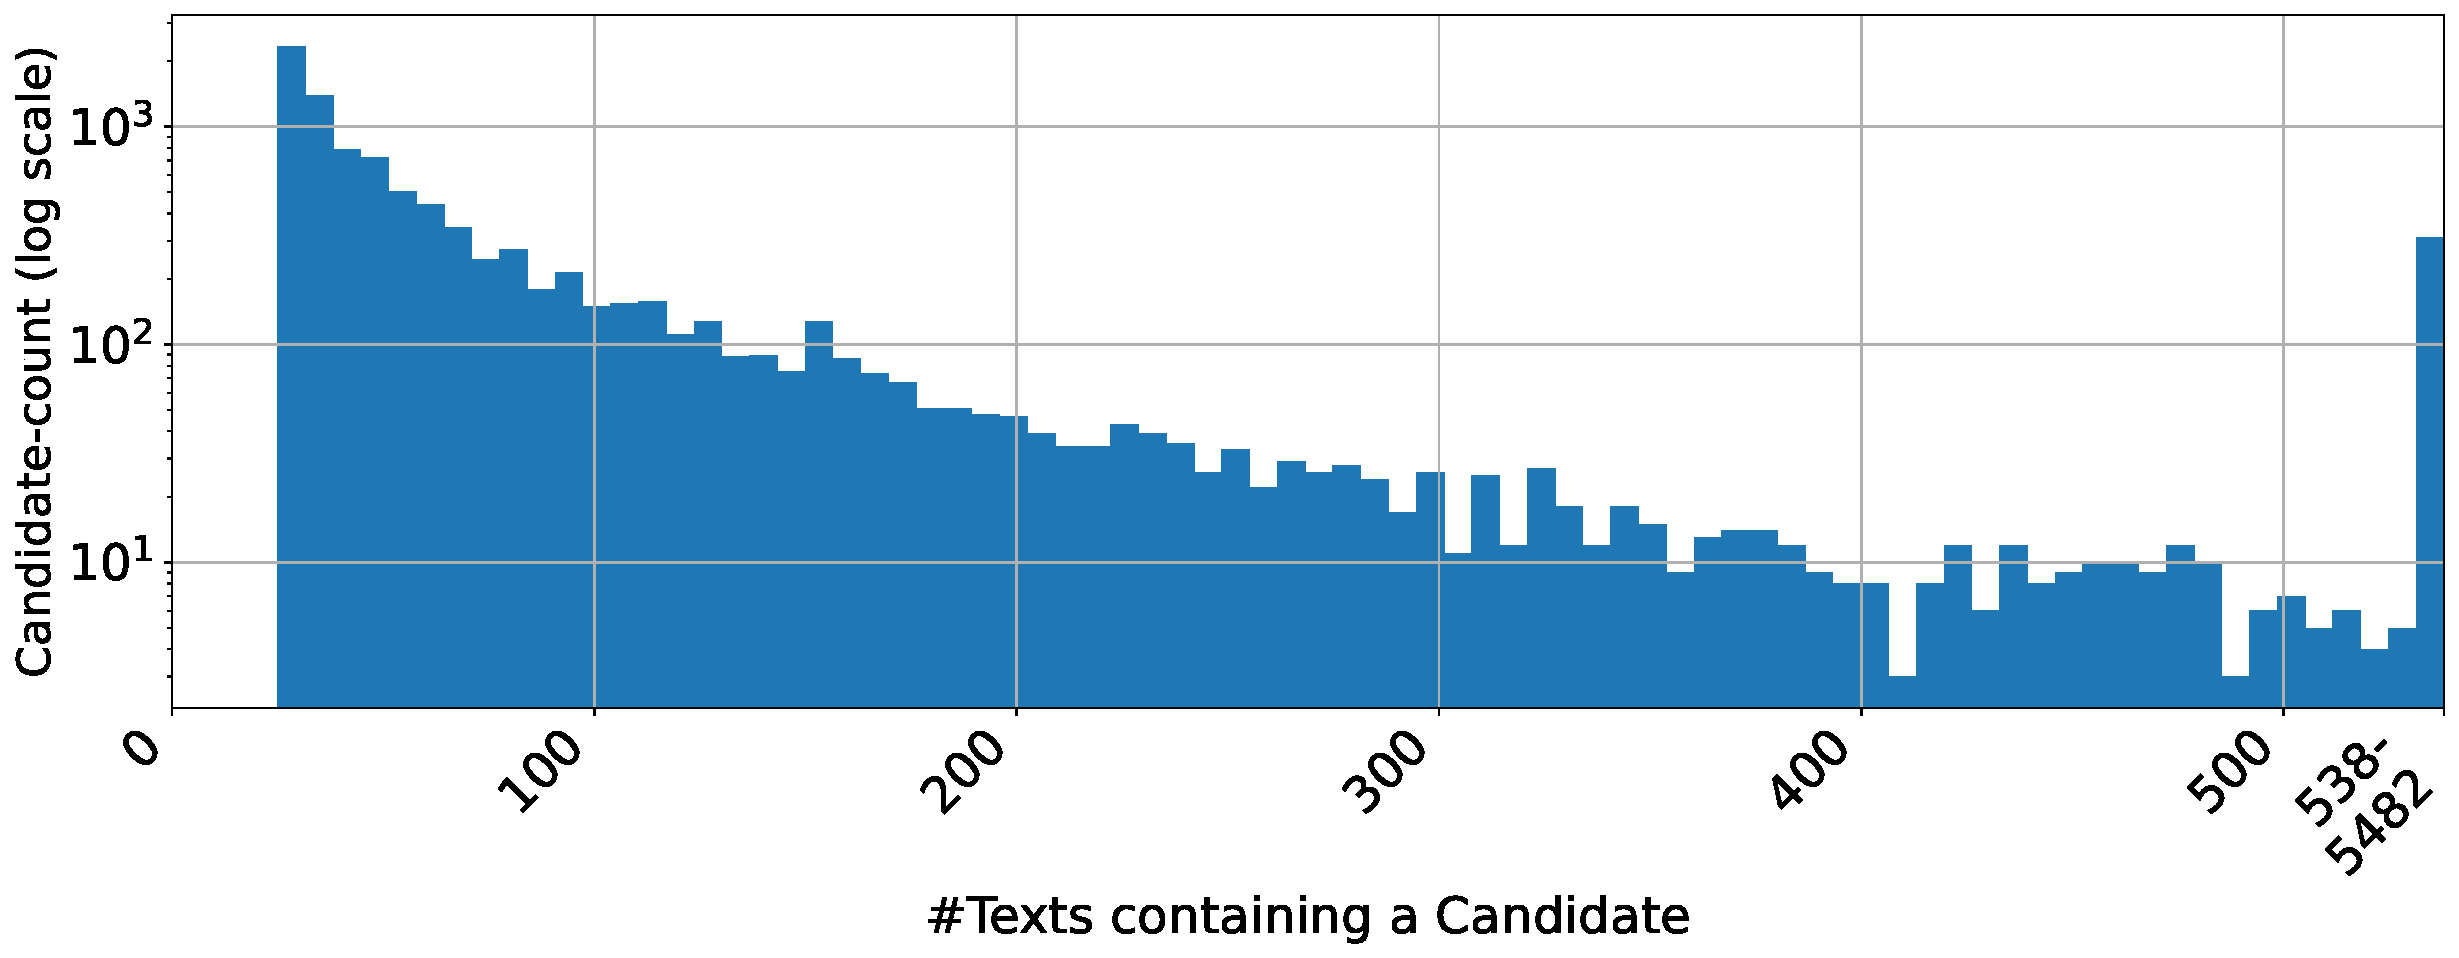
\includegraphics[width=\figwidth]{graphics/dataset_new/docs_per_phrase.pdf}
	\caption[Distribution of texts per candidate.]{Distribution of texts per candidate (log scale), cut off at the 97\textsuperscript{th} percentile. \Gls{df}-threshold for a candidate is set to 25, yielding 10\,060 candidates for 11\,601 documents. Median number of documents per candidate is 49 and for the 95\textsuperscript{th} percentile 375. 2595 candidates occur in at least 100 descriptions.}
	% Occurences in all Documents per Keyphrase (for all keyphrases that occur $\geq$ 5 times, cut off at the 93th percentile). 7007 of 45295 terms occur at least 5 times. Most frequent phrases: seminar (4173), course (3722), students (2923), it (2671), language (2071), work (1980), event (1842), research (1731), lecture (1723), law (1719).
	\label{fig:candidate_histogram}
\end{figure}

These results show that the algorithm produces much less candidates for our dataset compared with the originally considered ones. Because of that, the subsequent steps of the algorithm have a less rich representation to choose from, decreasing the chance to achieve good performances downstream.

\section{Results for the Siddata-dataset}
\label{sec:results_siddata}

% \todoparagraph{The plots here show the results from several different parameter-configurations. Because of that, the extracted semantic directions and also the metrics may differ between the plots. This is not a bug but a feature - they are all differnent but all are nice}

As previously described, the primary method used here to check if the described methodology works for the domain of educational resources is to check if low-depth decision trees trained on the extracted semantic directions of the Siddata-dataset can classify a courses' faculty. Before doing that however, it is important to first validate if it can reasonably assumed that the faculty \textit{can generally} be extracted from only the descriptions associated with the entities.

\subsection*{Extracing faculties without the algorithm}

\begin{figure}[h]
	\begin{center}
	  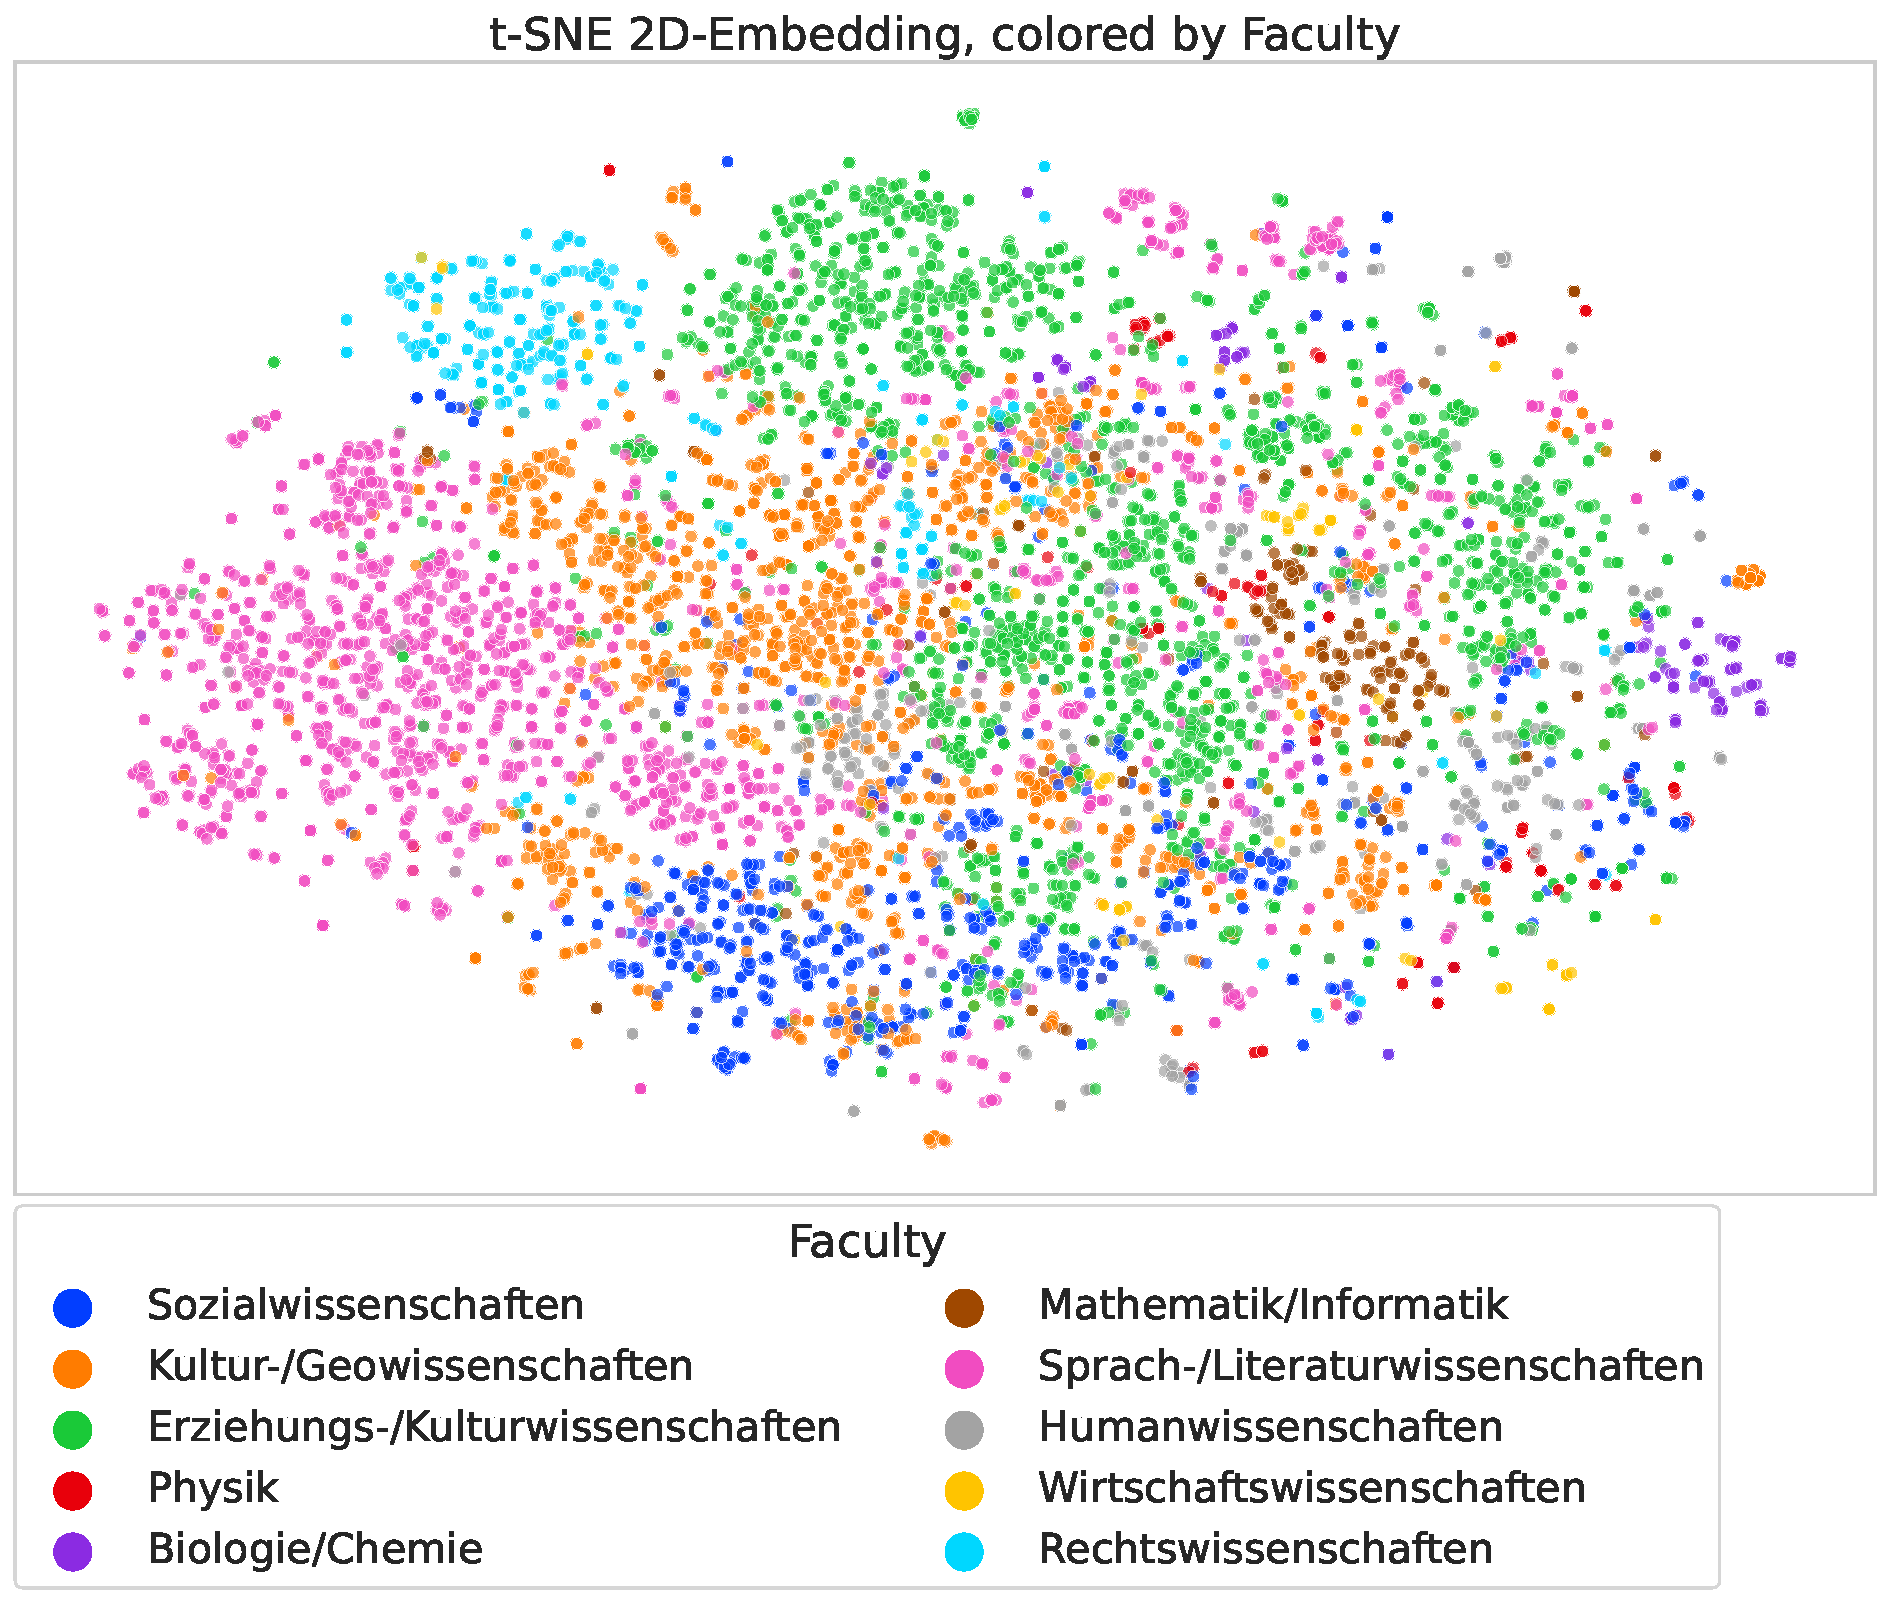
\includegraphics[width=0.9\textwidth]{graphics/dataset_new/scatter_mds_tsne_e2a70a9bf2.pdf}
	  \slcaption{2D Visualization of the Course-dissimilarity matrix, generated with \gls{tsne}. See \url{https://github.com/cstenkamp/derive_conceptualspaces/blob/main/notebooks/text_referenced_plots/visualise_embeddings.ipynb} for the origin of this plot as well as a 3D-plot on unaltered 3D-MDS-data that does not rely on t-SNE.}
	  \label{fig:scatter_mds_siddata}
	  % möchte sagen: Die Embeddings Clustern -> es lassen sich "sinnvolle Sachen" (wie faculty) draus ziehen.
	\end{center}
\end{figure}

To see if it is possible to extract any kind of structured data from the unstructured course descriptions, a \gls{bert}-based Neural Network classifier was trained on the dataset, classifying the subset of courses that are for the \gls{uos} to the faculty they belong to. The architecture of the classifier is described in Appendix~\ref{sec:faculty_classifier}.

The classifier trained for 12 epochs before \emph{stopping early} due to its performance on the test-set decreasing. It achieved an accuracy of \textbf{85.19\%} for the test-set (94.13\% on the training set), providing strong indication that the faculty can be considered a latent property of its description. Because \gls{bert} is one of the best general language classifiers to date \cite{Devlin2019}, this accuracy will be considered the upper boundary for the results of our algorithm.

\autoref{fig:scatter_mds_siddata} displays a \gls{tsne}-representation of the dissimilarity matrix generated from the normalized angular distances (\autoref{eq:norm_ang_dist}) of the \gls{bow}-representations generated from the courses (only those from the \gls{uos}) A first comparison of this scatter-plot and its placetypes-counterpart (\autoref{fig:scatter_mds_placetypes}) reveals that Siddata appears to have more homogenous clusters.

From this distance matrix, the algorithm subsequently creates an embedding using the \gls{mds}-algorithm to afterwards train multiple \glspl{svm} for each of the extracted candidate-dimensions before re-embedding the entities into a new space where the dimensions encode the \gls{rank} for each of the extracted features. To evaluate the algorithm, we will check if it is to be able to classify the faculty with a decision tree that uses between one and maximally $2^3=8$ of these features. To provide a context for the resulting performance, we will first look at a classification which does not use the feature-based representation, but a raw low-dimensional embedding without class-specific dimensions. This can be seen as the lower boundary of what a classification without selecting the most relevant dimensions but instead use an optimal but general three-dimensional space can achieve. A classification-performance of low-level decision trees that use only the most important features from all available ones that is higher than this thus provides evidence that the detected features encode important distinctive properties. \autoref{fig:mds_3d_hyperplane} visually represents the result of the classification using a linear \gls{svm} on a three-dimensional space generated as result of \gls{mds} on the dissimilarity matrix of the entities. Averaged over all Faculties, this classifier reaches a weighted accuracy of 64.3\% (unweighted accuracy 69.0\%, weighted F1: 0.414, unweighted F1: 0.269). Note that these values are reached by training on the full data without a separate testing-set.

% text_referenced_plots/siddata_analysis/visualise_embeddings_mds.ipynb


\begin{figure}[h]
	\begin{center}
	  \makebox[\textwidth][c]{
		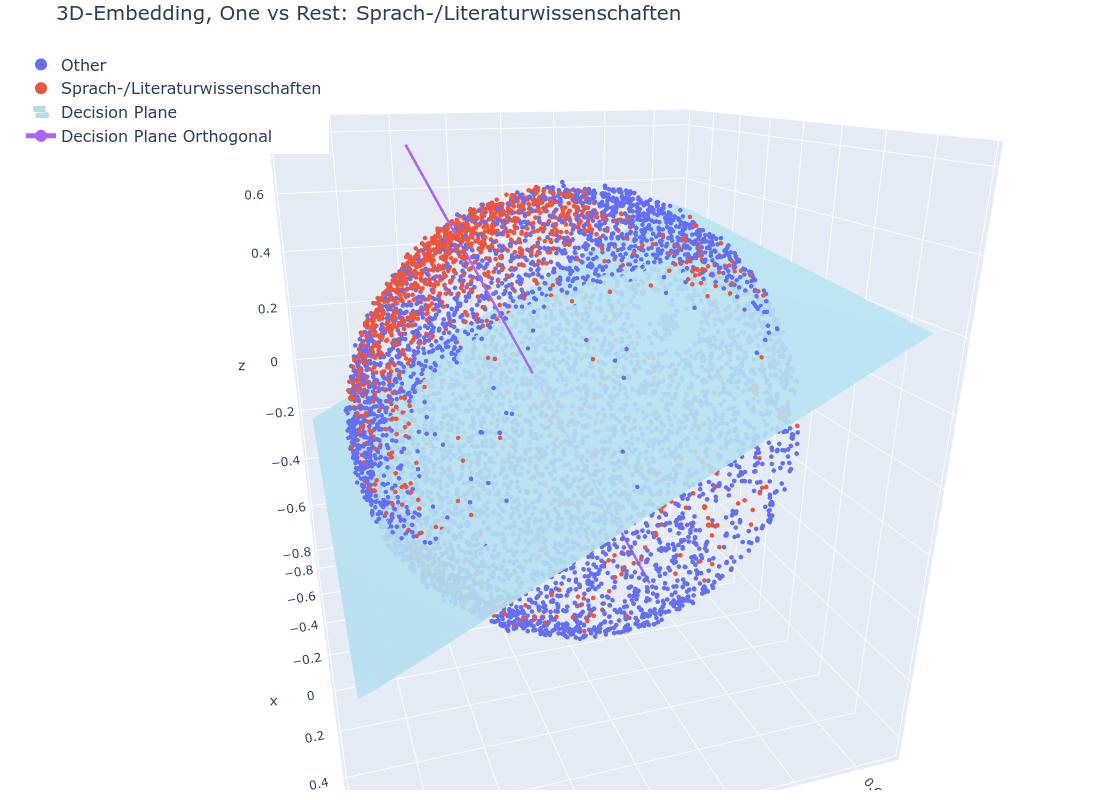
\includegraphics[width=1.1\textwidth]{graphics/dataset_new/possibledecision_sprachlit.png}
		\slcaption{A possible Hyperplane on a 3-Dimensional Embedding. The SVM depicted here reaches an Accuracy of 67.9\% (Precision: 39.8\%, Recall: 70.5\%). visualise interactively: \url{https://github.com/cstenkamp/derive_conceptualspaces/blob/main/notebooks/text_referenced_plots/visualise_embeddings_mds.ipynb} }
		\label{fig:mds_3d_hyperplane}
		%möchte sagen: To say what the lower boundary of what a 3D-Embedding of NON-CLASS-SPECIFIC dimensions can yield for classification, 
		% wie related der space von fig:boxes_rechtswis mit den interpretable dimensions zu IRGENDEINEM 3D-Space
	  }
	\end{center}
\end{figure}



\vspace{0.9ex}
\textbf{\large Extracing faculties with \glspl{dt} based on the 
algorithm}
\vspace{0.2ex}

Having established upper and lower boundary for what can reasonably be expected from the algorithm, let us finally look at the performance of its decision-trees, to gain evidence if human concepts are encoded in its extracted features. \autoref{tab:robustresults_perfb} lists average accuracies per faculty for decision trees created on the basis of a single hyperparameter-configuration that was selected to achieve high performance on average. The respective values are the average and standard-deviation of runs with 5-fold crossvalidation each for trees of various depths. The results show high accuracies across all faculties even for low-depth trees, but the faculty \textit{Humanwissenschaften} displays a high standard deviation for that condition.

\begin{table}[H]
	\begin{tabular}{rccccc}
		\toprule
		\textbf{Depth} &  \textbf{1} & \textbf{2} & \textbf{3} & \textbf{any} \\
		\midrule
		\textbf{Accuracy} & 0.056 ± 0.008 & 0.078 ± 0.042 & 0.196 ± 0.017 & 0.584 ± 0.015 \\
		\textbf{F1}       & 0.072 ± 0.006 & 0.125 ± 0.014 & 0.199 ± 0.007 & 0.513 ± 0.020 \\
		\bottomrule
	\end{tabular}
	\caption[Robust scores for classifying all faculties at once.]{Robust scores of a well-performing configuration for classifying all faculties at once. The reported results are mean and standard deviation from the result of ten runs with 5-fold crossvalidation each.}
	\label{tab:robustresults_allatonce}
\end{table}


\begin{table}[H]
	\resizebox{\textwidth}{!}{%
		\begin{tabular}{rcccc}
		\toprule
		\textbf{Depth} & \textbf{1} & \textbf{2} & \textbf{3} & \textbf{unbound} \\
		\midrule
		\textbf{Sozialwissenschaften} & 0.831 ± 0.021 & 0.811 ± 0.033 & 0.780 ± 0.028 & 0.918 ± 0.006 \\
		\textbf{Kultur-/Geowissenschaften} & 0.806 ± 0.010 & 0.728 ± 0.066 & 0.813 ± 0.022 & 0.873 ± 0.008 \\
		\textbf{Erziehungs-/Kulturwissenschaften} & 0.791 ± 0.010 & 0.824 ± 0.010 & 0.828 ± 0.020 & 0.868 ± 0.008 \\
		\textbf{Physik} & 0.747 ± 0.054 & 0.770 ± 0.033 & 0.818 ± 0.038 & 0.983 ± 0.003 \\
		\textbf{Biologie/Chemie} & 0.787 ± 0.044 & 0.838 ± 0.049 & 0.890 ± 0.036 & 0.982 ± 0.004 \\
		\textbf{Mathematik/Informatik} & 0.866 ± 0.031 & 0.844 ± 0.051 & 0.882 ± 0.038 & 0.978 ± 0.004 \\
		\textbf{Sprach-/Literaturwissenschaften} & 0.832 ± 0.009 & 0.832 ± 0.009 & 0.862 ± 0.009 & 0.902 ± 0.008 \\
		\textbf{Humanwissenschaften} & 0.630 ± 0.130 & 0.768 ± 0.103 & 0.781 ± 0.093 & 0.949 ± 0.005 \\
		\textbf{Wirtschaftswissenschaften} & 0.903 ± 0.015 & 0.910 ± 0.034 & 0.924 ± 0.018 & 0.989 ± 0.003 \\
		\textbf{Rechtswissenschaften} & 0.948 ± 0.031 & 0.894 ± 0.015 & 0.952 ± 0.011 & 0.985 ± 0.003 \\
		\textbf{Mean (weighted)} & 0.814 ± 0.035 & 0.822 ± 0.040 & 0.853 ± 0.031 & 0.943 ± 0.005 \\
		\textbf{Mean (unweighted)} & 0.810 ± 0.020 & 0.806 ± 0.031 & 0.835 ± 0.023 & 0.901 ± 0.007 \\
		\bottomrule
		\end{tabular}
	}
	\slcaption{Robust accuracies per faculty of a well-performing configuration. The reported results are mean and standard deviation from the result of ten runs with 5-fold crossvalidation each.\hideref{tab:robustresults_perfb_f1}{F1-Table}}
	\label{tab:robustresults_perfb}
\end{table}

Keep in mind that accuracies often make the situation look better than it is. The weighted average F1-scores are between 0.505 (depth 1) and 0.710 (unbounded). For the full table of F1-scores it is referred to the appendix, specifically \autoref{tab:robustresults_perfb_f1}. 

Compared with the results of the \gls{bert}-based classifier (85.19\%), the achieved results are suprisingly competitive, with the weighted mean of trees of depth one and two only slighly below that, and deeper trees achieving even higher accuracies. 
% "suprisingly competitive" ersetzen mit "soundso ist der przentsatz, soundso ist unserer, wir observen soundsoeinen unterschied"
% \todoparagraph{We said in the previous section that there are less candidates, making it harder. These quantifiable results show that it appears to work anyway.}  % "wie in 4.2 gibts weniger candidates, was es downstream schwieriger macht, aber wie in 4.3 klappts ja trotzdem." => Das geht selbst in results, da es eine quantifizierbare darstellung von verhältnismäßigkeiten ist und keine bewertung
Importantly however, the results reported here are those of a sepearate classifier per faculty (\textit{1vsRest}), differentiating only between the respective faculty as positive class and all other faculties as negative class. As will be further elaborated in the discussion, this is the only realistic way of doing it: A binary tree of depth one can differentiate between maximally two classes and thus maximally achieve a classification by perfectly classifying the most frequent class and labelling all samples as the second most frequent class, which in the case of faculties is $(2011+1665)/7081=51.9\%$. Results for such trees are reported in \autoref{tab:robustresults_allatonce}.



\subsubsection{Recovering entities from salient directions}
\label{sec:duplicate_maps}

After having tested if our semantic embedding captures at least one prominent latent topic of the data, we will additionally check if the produced embedding adequately captures enough of the general variability of the data. For that, we check if it is possible to recover entities from the salient directions, to ensure that no important relevant information was lost when mapping them to their semantic embedding. To get a general understanding, let us consider under what circumstances multiple different entities will fall towards the exact same coordinates. 

To get an estimate of the importance of each dimension of the embedding, we started with a full matrix where each entity is defined via each semantic direction. Starting with a 200-dimensional space, we removed random directions. Further we applied different levels of discretisation to the remaining dimensions. We wondered what amounts of discretisation and removal of dimensions is necessary for multiple entities to fall onto the same category. Each combination was done multiple times, each time removing other random directions, and the percentage of duplicates in the data was counted. \autoref{tab:duplicates_per_comb} displays the result of this.

\begin{table}[h]
	\caption[Duplicates per combination of dimensionality and discretisation-categories.]{Duplicates per combination of dimensionality and amount of categories per left-over category. Row = number of left-over dimensions, cols = discretisation (number in parantheses is the divisor of the orginal value)}
	\begin{tabular}{lrrrrrr}
	\toprule
	 & \textbf{2} & \textbf{11} & \textbf{23} & \textbf{116} & \textbf{232} & \textbf{1160} \\
	\#dims & (5800) & (100) & (50) & (10) & (5) & (2) \\
	\midrule
	3 & 100\% & 99.85\% & 68.98\% & 6.85\% & 5.25\% & 3.97\% \\
	5 & 100\% & 24.91\% & 9.79\% & 5.25\% & 4.72\% & 3.42\% \\
	10 & 100\% & 10.18\% & 6.90\% & 4.67\% & 4.23\% & 2.11\% \\
	20 & 100\% & 7.41\% & 5.58\% & 4.23\% & 3.52\% & 0.79\% \\
	50 & 99.97\% & 5.46\% & 4.72\% & 3.19\% & 1.89\% & 0.05\% \\
	100 & 99.88\% & 4.80\% & 4.18\% & 1.94\% & 0.65\% & 0\% \\
	200 & 99.55\% & 4.36\% & 3.44\% & 0.67\% & 0.09\% & 0\% \\
	\bottomrule
	\end{tabular}
	\label{tab:duplicates_per_comb}
\end{table}


\subsection{Qualitative Analysis}

The main goal of the algorithm is not to optimally classify the respective faculties, but to find semantic directions. Thus, once it has been established that the performance is reasonably well, looking at the names of these directions is just as important. \autoref{fig:dims_for_fb} visually represents decision-trees for each of the faculties of depth one, \ie trees that can only use a single semantic direction for their decision. With the exception of the faculties \emph{Physik} and \emph{Biologie/Chemie}, the semantic directions that best predict each faculty appear very relevant to the respective topic.

\begin{figure}[h]
	\begin{center}
	  \makebox[\textwidth][c]{
		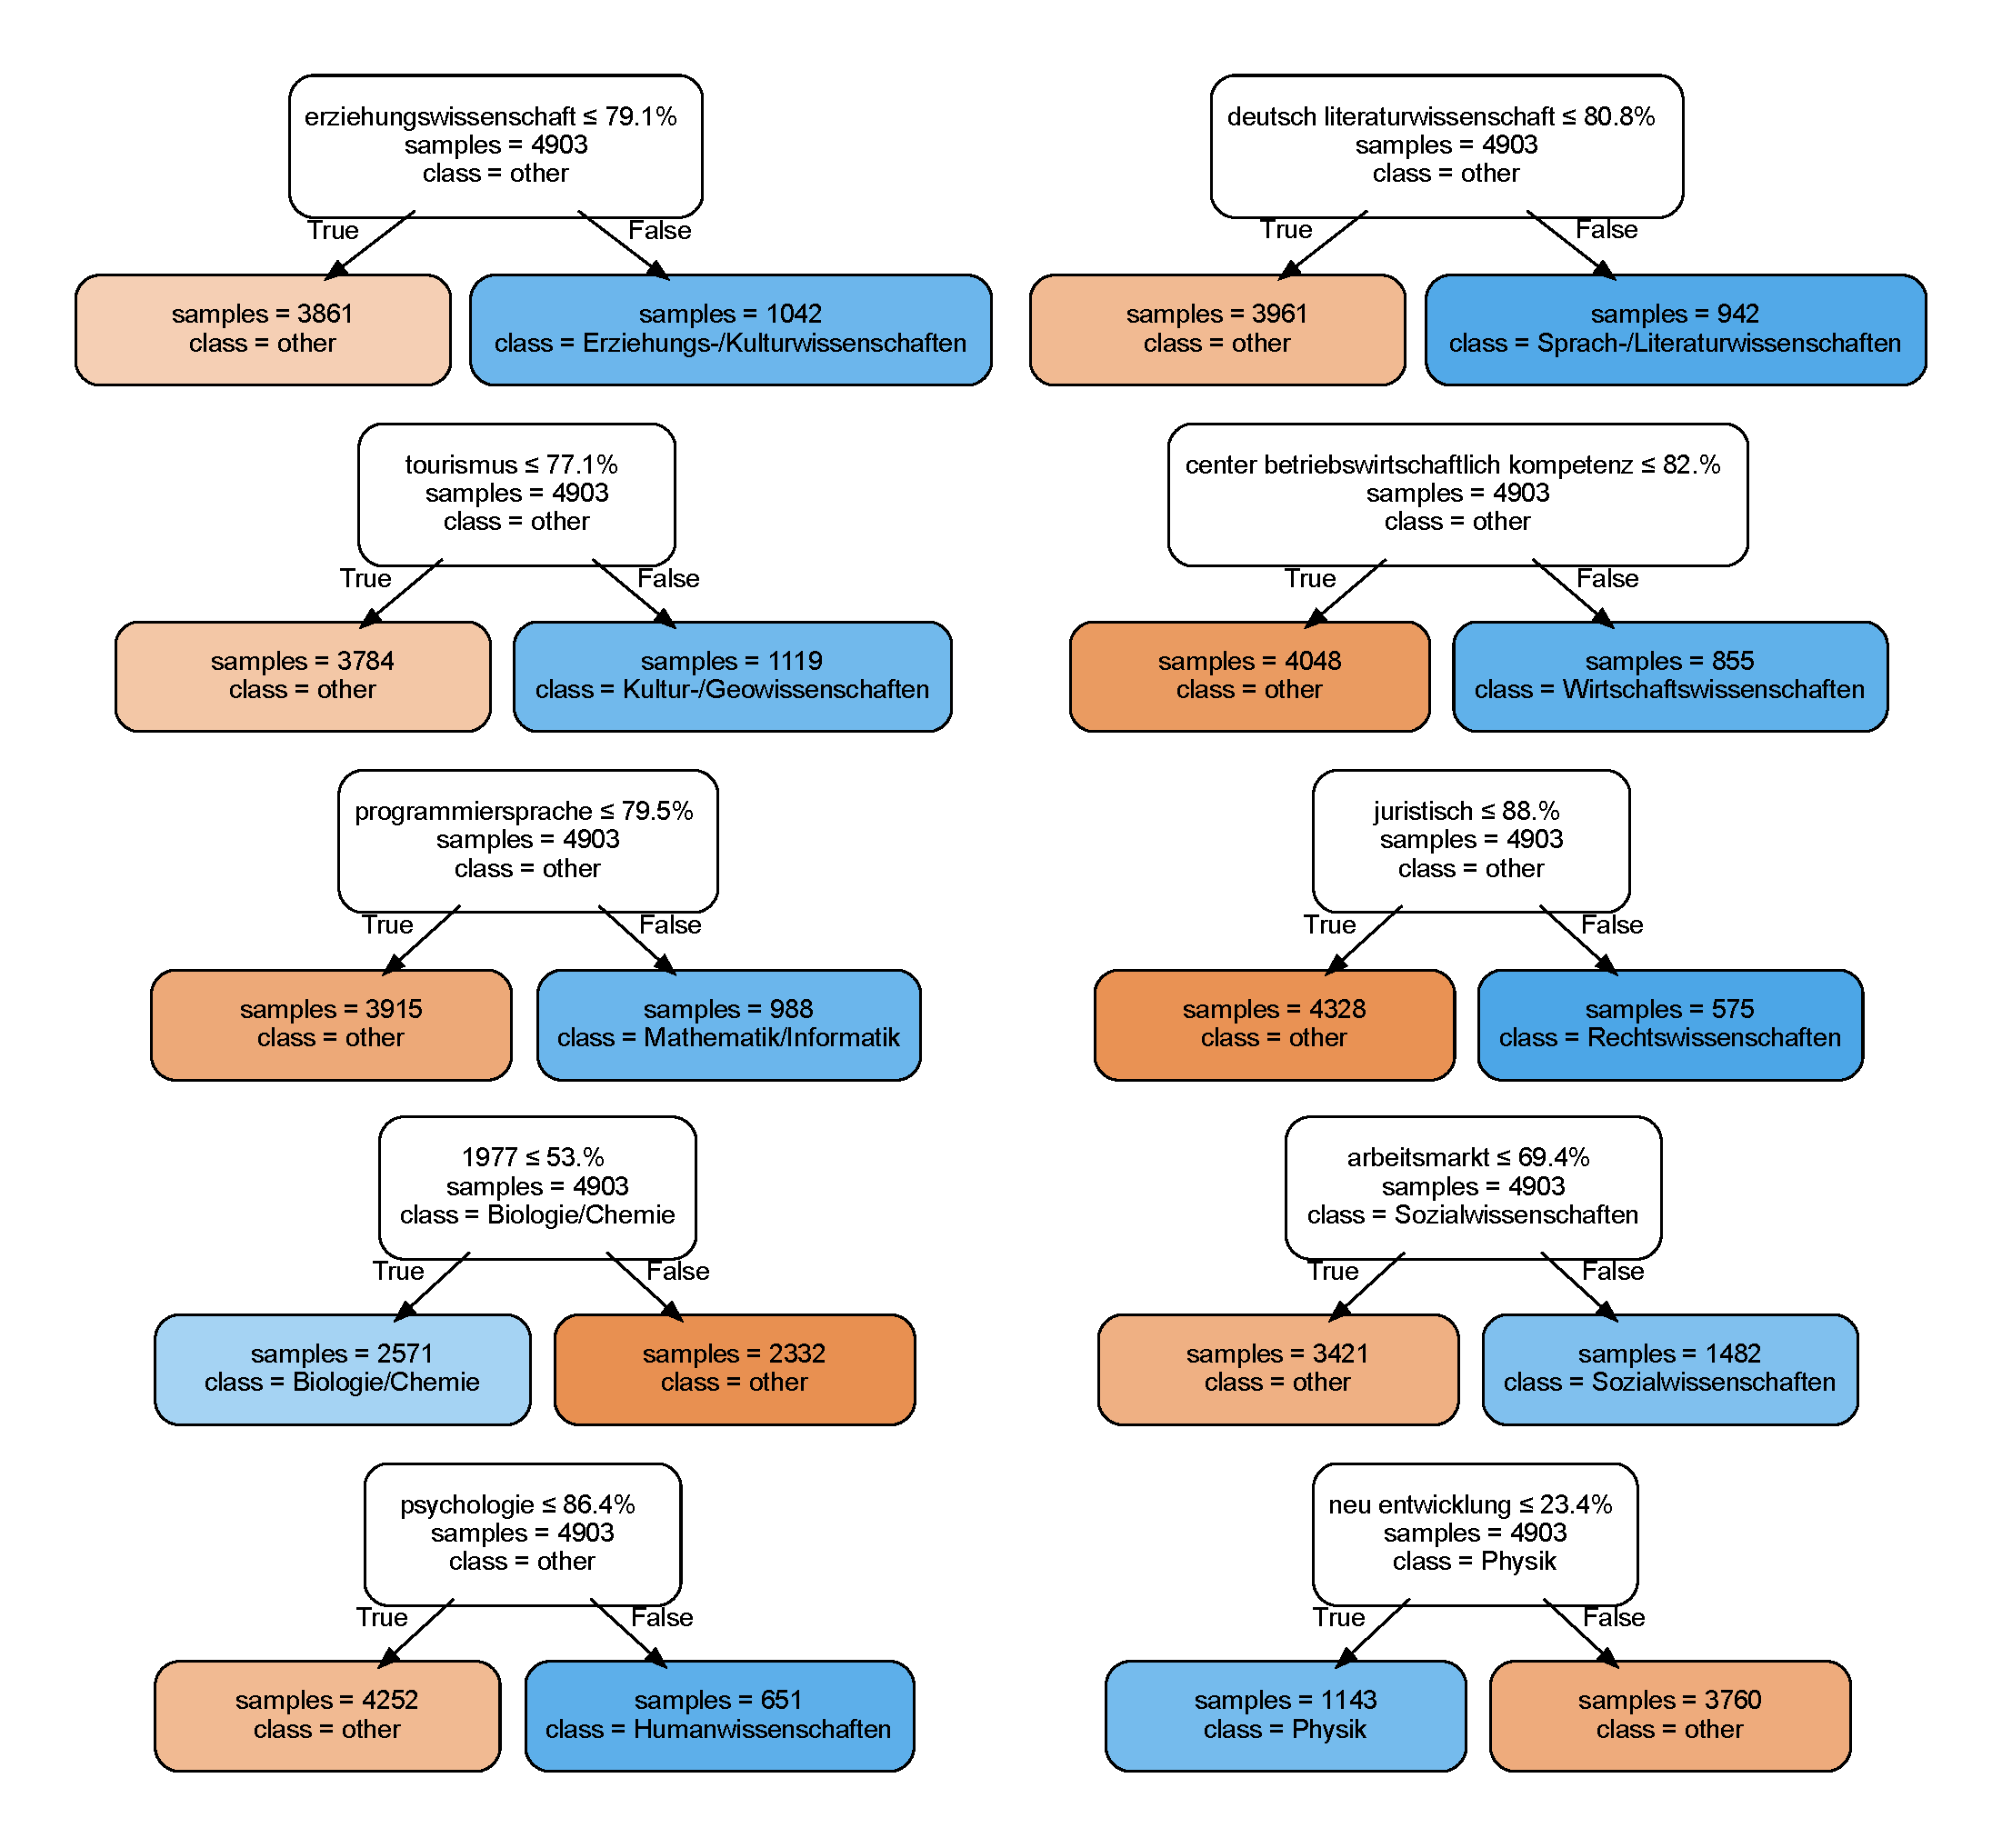
\includegraphics[width=1.3\textwidth]{graphics/dataset_new/dims_for_fb.pdf}
		\slcaption{Resulting \glspl{dt} with only a single decision for each of the faculties. The white boxes show a semantic direction and the maximal rank \wrt to this direction for an entity to fall under the class designated by the respective left branch.}
		\label{fig:dims_for_fb}
		% möchte sagen: Unsere Extracted Dimensions entsprehcen human concepts wie Fachbereich
	  }
	\end{center}
\end{figure}

For trees deeper than one level, the selected features from the second level on are not necessarily the most important ones.\footnote{A \gls{dt} has separate conditions for every subtree, which means on level two there are two different features that depend on the result of the first split.} Instead it is possible to extract the most important features for a classification by looking at the respective information gain achieved by splitting it. \autoref{tab:courses_top3} displays the resulting three most important directions for each of the respective faculties. While the details of this result will be eloborated upon in the discussion, most of the detected features appear convincing. Regarding an actual classification using these features, \autoref{fig:boxes_rechtswis} in the Appendix displays the result of a sample classification of a decision tree with three features.


\begin{table}[H]
	\makebox[\textwidth][c]{
		\resizebox{1.1\textwidth}{!}{%
		\setlength{\tabcolsep}{2pt}
		\begin{tabular}{r@{\hskip 8pt}lllcr@{\hskip 6pt}c}
		& & & & \multicolumn{2}{c}{\textbf{Accuracy}} \\
		\textbf{Faculty} & \multicolumn{3}{c}{\textbf{Top 3 Directions}} & \textbf{Top 3} & \textbf{Top 1} \\
		\midrule
		\textbf{Erziehungs-/Kulturw.} & erziehungswissenschaft & okumenisch & english for & 78.02\% & 75.50\% \\
		\textbf{Rechtswissenschaften} & juristisch & bgb & bgb & 95.86\% & 91.10\% \\
		\textbf{Wirtschaftsw.} & {\scriptsize center betriebswirtschaftlich kompetenz } & religionsunterrichts & design & 89.65\% & 79.10\% \\
		\textbf{Kultur-/Geow.} & tourismus & gi & stadtgeographie & 75.50\% & 77.44\% \\
		\textbf{Mathem./Informatik} & programmiersprache & menge & hoffnung & 93.00\% & 91.85\% \\
		\textbf{Sprach-/Literaturw.} & deutsch literaturwissenschaft & sprache & okumenisch & 86.71\% & 85.10\% \\
		\textbf{Humanwissenschaften} & psychologie & metaphysik & internationalisierung & 86.84\% & 85.51\% \\
		\textbf{Physik} & neu entwicklung & mitarbeiterinnen & {\small regelmassig aktiv teilnahme} & 78.27\% & 77.36\% \\
		\textbf{Biologie/Chemie} & aktivierung studierend & brd & berucksichtigung finden & 85.22\% & 62.13\% \\
		\textbf{Sozialwissenschaften} & arbeitsmarkt & regieren & multiple & 78.60\% & 67.63\% \\
		\end{tabular}
		\slcaption{Top 3 directions to detect the respective faculty from the data. Note that it may also be the case that low values for the respective feature encode class membership.}
		\label{tab:courses_top3}
		}
	}
\end{table}


\newcolumntype{L}[1]{>{\raggedright\let\newline\\\arraybackslash\hspace{0pt}}m{#1}}
\newcolumntype{C}[1]{>{\centering\let\newline\\\arraybackslash\hspace{0pt}}m{#1}}
\newcolumntype{R}[1]{>{\raggedleft\let\newline\\\arraybackslash\hspace{0pt}}m{#1}}



\begin{table}[h]
	\centering
	\makebox[\textwidth][c]{
		\resizebox{1.1\textwidth}{!}{%
	\begin{tabular}{R{0.2\textwidth}|L{0.9\textwidth}}
	   Cluster Center & Cluster Elements \\ \midrule
				 opnv & befragungen, bewohner, urbanen, 00 uhr \\
	   bertolt brecht & brecht, exil, bertolt, weiss, weimarer republik, auschwitz, weimarer, ... \\
religionswissenschaft & religionsunterrichts, spirituelle, religions, teil veranstaltung, religion, studienbeginn, auml ischen, ... \\ 
		 erkrankungen & klinischen, gesundheitlichen, krankheit, rehabilitation, pravention, aufrechterhaltung, exemplarische inhalte, ... \\
	  		  lineare & integrierte, berechnung, variablen, skript, ubungsaufgaben, losung, vorliegen \\
	 		 parteien & verfassung, demokratischen, zivilgesellschaft, semester sowie, einander, folgendem link, sozialwiss uni osnabrueck, ... \\
	 		 kleidung & textilien, mode, textile, parallelen \\
			    kreuz & heilige, christentum, 1957, fuhrungen \\
 		 offentliches & offentlichkeitsarbeit, verwaltungsrecht, offentlichen recht, offentliches recht, europarecht, staatsrecht, teilnahmevoraussetzungen veranstaltung, ... \\
	    masterstudium & fortgeschrittene, schlusselkompetenzen, betriebswirtschaftslehre, untereinander \\
	unterrichtspraxis & fachlichen, unterrichtsplanung, schulalltag, lehrerinnen, schulische, daz, bildung nachhaltige, ... \\
  		  aristoteles & asthetik, semantik, dialoge, menschheit, sucht, benutzt, philosophische, ... \\
   		   mythologie & athen, mythos, mann, griechen, ubersetzung, figur, griechischen, ... \\
 		 flexibilitat & weiterbildung, schlusselqualifikation, erfolgreiches, fordert, vorlagen, strukturierte, berufsleben, ... \\
   aktive beteiligung & teilnahme ersten, wochentliche, zweit, festlegung, ubergreifende, auml ndige, ndige, ... \\
 		 unsicherheit & covid 19 pandemie, korperlich, wendet studierende, webinar, risiko, einbringen, fachlich, ... \\
	 wirtschaftlicher & industrialisierung, wachstum, republik, wirtschaftspolitik, konkurrenz, positive, russland, ... \\
	\end{tabular}
	}}
	\caption{Exemplary clusters found in the Siddata-dataset.}
	\label{tab:clusters}
\end{table}	


% \removeMe{
% \subsubsection{Are the phrases making up the semantic-direction-clusters similar?}
% \todo
% \subsubsection{Are there dimensions encoding the COVID-19 pandemic?}
% \todo
% \subsubsection{Is there a direction capturing advanced courses?}
% \todo
% }



% \subsubsection{Extended analysis}
% \removeMe{
% \todoparagraph{Also interesting: The top-ranked entities for some of the features }

% \todoparagraph{Neben den Clustern die ich mir anzeigen lassen kann und qualitativ analysieren kann}, kann ich mir auch die distances to the origins of the respective dimensions (induced by the clusters), what induces the respective rankings! (see DESC15 p.24u, proj2 of load_semanticspaces.load_projections) anzeigen lassen - da kann ich sagen "term xyz ist bei "nature" am höchsten".
% }




\origsection{Optimal Parameters}
\label{sec:results_params}

Having established the algorithm's ability to be transferred to the domain of educational resources, we will conclude this chapter with the results of our hyperparameter search. The algorithm was run with hundreds of different hyperparameter-combinations for both the placetypes- and Siddata-dataset throughout the process of its implementation and testing. As the precise hyperparameter-combination was not very imporant for our research questions, only some exemplary results for the Siddata-dataset will be reported here for the sake of brevity.

The reports produced in the previous section are the best ones from a final set of 165 different parameter-combinations, run over the course of three days on the \gls{ikw}-grid. % \todoparagraph{which was in contrast to the mainalgos easy thanks to my scalable implementation hehe} 


Generally, we selected a parameter-configuration that reached a high accuracy on average for the aforementioned classifiation based on shallow decision trees as representatively \textit{good} configuration. Here we compare all of the parameter-combinations that were considered - however the printed tables are shortened for a clearer overview.

As described in \autoref{sec:svm_filter_cands}, a good first approximation for the quality of an embedding is to check how many candidate-terms get a kappa-score which is above the threshold of $0.5$. Unfortunately, \cite{Derrac2015} and its follow-ups \cite{Ager2018,Alshaikh2020} did not explictly and unambiguously state how the kappa-score was calculated. Not only does its implementation have many arguments, but also the application may vary. In general, it compares the \textit{prototypicality} according to the classificiation decision with the \gls{quant} of how often the according word occurs in the entities' associated texts. The precise mechanism of has however many more parameters: for example, one can only consider those entities that have a positive \gls{quant}-score, such that not almost all of the candidates have a score of zero\footnote{For the movies-dataset, a \gls{df} threshold of 100 for a candidate means that up to 14\,900 entities (99.33\%) do not contain the entities, meaning all scores and accordingly also their rank will be zero. In constrast to that, the ranking induced by mapping of the high-dimensional and real-valued embeddings onto the separatrix orthogonal will almost always lead to unique ranks.}. Another open question is when considering the raw count as quantification\footnote{The exact wording of \textcite{Derrac2015} is: \textit{\q{[...] measure the correlation between the ranking induced by \vec{v_t} and the number of times t appears in the documents associated with each entity [...]}}. This seems to imply that they are using the raw count, even though \cite{Ager2018,Alshaikh2020} write in their algorithm summary that they used the \gls{ppmi}-score}, if the rankings induced by the orthogonal of the hyperplane are to be compared with the raw count, or the \textit{ranking induced} by the count. To clarify this ambiguity, we tried out many different interpretations for this score. 

\autoref{tab:kappa_table} (moved to the Appendix) shows the results of many runs with different parameter-combinations with the purpose of figuring out which combination of parameters and kappa-metrics lead to enough candidate-terms. The meaning of the different kappa-scores encoded in the columns is given in the implementation details in \autoref{tab:kappa_measures}. \todoparagraph{Also ref the figure of workflow where we check what threshold was realistic}. The table shows drastically differing values for the individual scoring methods. To understand if the difference in scoring has an effect on \textit{which} candidates are extracted, let us look at the overlap of different measures in \autoref{tab:kappa_overlap}. 
% \todoparagraph{Zeigt er hier ?? ?}


\begin{table}[H] 
	\resizebox{\textwidth}{!}{%
	\begin{tabular}{rccccccccccccc}
		\toprule
		 & \textbf{accuracy} & \textbf{precision} & \textbf{recall} &  \textbf{f1} & \textbf{r2r-d} & \textbf{r2r-min} & \textbf{b2b} & \textbf{dig} & \textbf{c2r+} & \textbf{r2r+d} & \textbf{r2r+min} & \textbf{r2r+max} & \textbf{dig+2} \\
		 & (10060) & (1668) & (10060) & (3155) & (0) & (2) & (3052) &  (0) & (4) & (0) & (239) & (103) & (1010) \\
		\midrule
		accuracy & - & 0.166 & \bfseries 1.000 & 0.314 & 0.000 & 0.000 & 0.303 & 0.000 & 0.000 & 0.000 & 0.024 & 0.010 & 0.100 \\
		precision & \bfseries 1.000 & - & \bfseries 1.000 & \bfseries 1.000 & 0.000 & 0.001 & 0.998 & 0.000 & 0.002 & 0.000 & 0.084 & 0.051 & 0.126 \\
		recall  & \bfseries 1.000 & 0.166 & - & 0.314 & 0.000 & 0.000 & 0.303 & 0.000 & 0.000 & 0.000 & 0.024 & 0.010 & 0.100 \\
		f1  & \bfseries 1.000 & 0.529 & \bfseries 1.000 & - & 0.000 & 0.001 & 0.967 & 0.000 & 0.001 & 0.000 & 0.067 & 0.032 & 0.140 \\
		r2r-d  & 0.000 & 0.000 & 0.000 & 0.000 & - & 0.000 & 0.000 & 0.000 & 0.000 & 0.000 & 0.000 & 0.000 & 0.000 \\
		r2r-min  & \bfseries 1.000 & \bfseries 1.000 & \bfseries 1.000 &  \bfseries 1.000 & 0.000 & - & \bfseries 1.000 & 0.000 & 0.000 & 0.000 & 0.000 & 0.000 & 0.000 \\
		b2b  & \bfseries 1.000 & 0.546 & \bfseries 1.000 & \bfseries 1.000 & 0.000 & 0.001 & - & 0.000 & 0.001 & 0.000 & 0.068 & 0.033 & 0.141 \\
		dig & 0.000 & 0.000 & 0.000 & 0.000 & 0.000 & 0.000 & 0.000 & - & 0.000 & 0.000 & 0.000 & 0.000 & 0.000 \\
		c2r+  & \bfseries 1.000 & \bfseries 1.000 & \bfseries 1.000 & \bfseries 1.000 & 0.000 & 0.000 & \bfseries 1.000 & 0.000 & - & 0.000 & \bfseries 1.000 & \bfseries 1.000 & 0.250 \\
		r2r+d  & 0.000 & 0.000 & 0.000 & 0.000 & 0.000 & 0.000 & 0.000 & 0.000 & 0.000 & - & 0.000 & 0.000 & 0.000 \\
		r2r+min  & \bfseries 1.000 & 0.586 & \bfseries 1.000 & 0.887 & 0.000 & 0.000 & 0.874 & 0.000 & 0.017 & 0.000 & - & 0.406 & 0.452 \\
		r2r+max  & \bfseries 1.000 & 0.825 & \bfseries 1.000 & 0.981 & 0.000 & 0.000 & 0.981 & 0.000 & 0.039 & 0.000 & 0.942 & - & 0.437 \\
		dig+2  & \bfseries 1.000 & 0.208 & \bfseries 1.000 & 0.438 & 0.000 & 0.000 & 0.426 & 0.000 & 0.001 & 0.000 & 0.107 & 0.045 & - \\
		\bottomrule
	\end{tabular}
	\slcaption{Overlap of different scoring methods in percent. Numbers in parantheses list the total number of extracted samples for each scoring method. Upper right triangle encodes the cardinality of the union divided by the cardinality of column-method, lower left triangle divides by row.}
	\label{tab:kappa_overlap}
	}
\end{table}
	
This table additionally reports the raw \textit{accuracy, precision, recall} and \textit{f1}-scores of the classifier. The overlaps of these scores will  serve to test our hypothesis that due to the different nature of the Siddata-dataset, comparing the \textit{ranking} of the candidates leads to worse performances than comparing raw classification scores (also suggested by \cite{Ager2018}).

After these preliminary analyses with the number of extracted candidates, let us also quickly look at differences in perforamances of the decision-trees depending on parameter-combinations. \autoref{tab:best_params} lists the accuracies of \glspl{dt} classifying a course's faculty per parameter-setup for some of the configurations of the final run. Specifically, this compares accuracies for several \textit{1vsRest} decision trees of depth one with a test-set size of 33\%.


\newcommand{\SmfauhcsdT}{\setlength\extrarowheight{-5pt} \scriptsize \mfauhcsdT}
\newcommand{\Smfauhtcsldp}{\setlength\extrarowheight{-5pt} \scriptsize \mfauhtcsldp}

% Other configs: {'dataset': 'siddata2022', 'debug': 'False', 'prim_lambda': '0.5', 'sec_lambda': '0.2', 'classifier_succmetric': 'kappa_digitized_onlypos_2', 'cluster_direction_algo': 'reclassify', 'kappa_weights': 'quadratic', 'embed_dimensions': '200', 'embed_algo': 'mds', 'quantification_measure': 'tfidf', 'dcm_quant_measure': 'count', 'extraction_method': 'tfidf', 'translate_policy': 'onlyorig', 'pp_components': 'mfauhtcsldp', 'language': 'de', 'min_words_per_desc': '80'}
% Args for best Tree: balance_classes=True, one_vs_rest=True, dt_depth=1, test_percentage_crossval=0.33
% \begin{table}[H]
% 	\resizebox{\textwidth}{!}{%
% 	\caption{Decision-Tree-Accuracies for different Parameter-Combinations}
% 	\label{tab:best_params}
% 	\begin{tabular}{lllrrrrrr}
% 	\toprule
% 	\multicolumn{3}{r}{\textbf{DTM-Quantification}} & \textbf{ppmi} &  &  & \textbf{tfidf} &  &  \\
% 	\textbf{Preprocessing} & \specialcell[b]{\textbf{Quanti-}\\ \textbf{fication}} & \textbf{Metric} &  &  &  &  &  &  \\
% 	\midrule
% 	\multirow[t]{7}{*}{\SmfauhcsdT} & \multirow[t]{3}{*}{count}   & k_c2r+ 	  & - 		& 40.58\% & 38.76\% & 36.24\% & 45.16\% & - \\
% 	 &  													     & k_dig+_2   & - 		& 74.83\% & 77.10\% & 74.82\% & 80.42\% & - \\
% 	 & 														     & k_r2r+_min & - 		& 73.59\% & 74.91\% & 77.58\% & 80.71\% & - \\
% 	\cline{2-3}
% 	 & \multirow[t]{2}{*}{ppmi} 							 	 & k_dig+_2   & 62.11\% & 58.63\% & 61.94\% & 79.97\% & - 		& - \\
% 	 & 													         & k_r2r+_min & 70.75\% & 75.52\% & 74.12\% & 81.10\% & - 		& - \\
% 	\cline{2-3}
% 	 & \multirow[t]{2}{*}{tfidf} 						         & k_dig+_2   & 57.86\% & 76.35\% & 76.88\% & 77.58\% & 80.49\% & - \\
% 	 &  													     & k_r2r+_min & 67.31\% & 73.45\% & 72.65\% & 77.17\% & 78.81\% & - \\
% 	\cline{1-3} \cline{2-3}
% 	\multirow[t]{7}{*}{\Smfauhtcsldp} & \multirow[t]{3}{*}{count} & k_c2r+	  & 49.72\% & 40.70\% & 41.94\% & 53.79\% & 49.17\% & 63.38\% \\
% 	 &  														 & k_dig+_2   & 58.25\% & 74.86\% & 77.67\% & 78.00\% & 79.73\% & 44.39\% \\
% 	 &  														 & k_r2r+_min & 66.51\% & 72.03\% & 69.78\% & 78.45\% & 79.15\% & 61.95\% \\
% 	\cline{2-3}
% 	 & \multirow[t]{2}{*}{ppmi}									& k_dig+_2 	 & - 		& - 	  & 65.67\% & 77.58\% & 80.08\% & 58.58\% \\
% 	 &  														& k_r2r+_min & - 		& - 	  & 80.41\% & \bst 81.41\% & \bst 81.41\% & 64.36\% \\
% 	\cline{2-3}
% 	 & \multirow[t]{2}{*}{tfidf} 								& k_dig+_2 	 & 64.88\% 	& 76.31\% & 77.81\% & 77.24\% & -  & 59.18\% \\
% 	 &  														& k_r2r+_min & 58.92\% 	& 78.05\% & 76.49\% & 77.09\% & -  & 63.02\% \\
% 	\bottomrule
% 	\end{tabular}
% 	}
% \end{table}


% Other configs: {'dataset': 'siddata2022', 'debug': 'False', 'prim_lambda': '0.5', 'sec_lambda': '0.2', 'classifier_succmetric': 'kappa_digitized_onlypos_2', 'cluster_direction_algo': 'reclassify', 'kappa_weights': 'quadratic', 'embed_dimensions': '200', 'embed_algo': 'mds', 'quantification_measure': 'tfidf', 'dcm_quant_measure': 'count', 'extraction_method': 'tfidf', 'translate_policy': 'onlyorig', 'pp_components': 'mfauhtcsldp', 'language': 'de', 'min_words_per_desc': '80'}
% Args for best Tree: balance_classes=True, one_vs_rest=True, dt_depth=1, test_percentage_crossval=0.33
\begin{table}
	\resizebox{\textwidth}{!}{%
	\slcaption{Decision tree accuracies for different parameter-combinations. (tree of depth 1, balanced, 1vsRest, 33\% testset)}
	\label{tab:best_params}
	\begin{tabular}{rrrrllllll}
	\toprule
	 &  \multicolumn{3}{r}{\textbf{Dimensions}} & \multicolumn{2}{l}{\textbf{3}} & \multicolumn{2}{l}{\textbf{50}} & \multicolumn{2}{l}{\textbf{200}} \\
	 &  \multicolumn{3}{r}{\textbf{Lambda$_2$}} & \textbf{0.1} & \textbf{0.2} & \textbf{0.1} & \textbf{0.2} & \textbf{0.1} & \textbf{0.2} \\
	 \textbf{Preprocessing} & \specialcell[b]{\textbf{Quanti-}\\ \textbf{fication}} & \specialcell[b]{\textbf{DCM}\\ \textbf{quant}} & \textbf{Metric} &  &  &  &  &  &  \\
	\midrule
	\multirow[t]{14}{*}{\textbf{\SmfauhcsdT}} & \multirow[t]{7}{*}{\textbf{ppmi}} & \multirow[t]{3}{*}{\textbf{count}} & {c2r+} & 53.24\% & 47.22\% & 48.36\% & 41.91\% & 40.87\% & 36.57\% \\
	 &  &  & {dig+2} & 49.66\% & 58.22\% & 74.73\% & 71.75\% & 80.32\% & 76.81\% \\
	 &  &  & {r2r+min} & 67.79\% & 65.09\% & 74.99\% & 72.61\% & 74.51\% & 73.72\% \\
	\cline{3-4}
	 &  & \multirow[t]{2}{*}{\textbf{ppmi}} & {dig+2} & 63.49\% & 64.76\% & 55.78\% & 61.40\% & 55.10\% & 65.32\% \\
	 &  &  & {r2r+min} & 62.43\% & 67.83\% & 75.30\% & 75.99\% & 76.97\% & 73.84\% \\
	\cline{3-4}
	 &  & \multirow[t]{2}{*}{\textbf{tfidf}} & {dig+2} & 55.81\% & 62.23\% & 75.22\% & 73.88\% & 76.34\% & 79.14\% \\
	 &  &  & {r2r+min} & 63.23\% & 62.35\% & 70.58\% & 72.60\% & 77.69\% & 72.75\% \\
	\cline{2-4} \cline{3-4}
	 & \multirow[t]{7}{*}{\textbf{tfidf}} & \multirow[t]{3}{*}{\textbf{count}} & {c2r+} & 44.99\% & 59.00\% & 60.27\% & 37.56\% & 56.05\% & 43.24\% \\
	 &  &  & {dig+2} & 45.45\% & 49.86\% & 75.75\% & 77.77\% & 76.25\% & 80.86\% \\
	 &  &  & {r2r+min} & 61.91\% & 63.94\% & 72.69\% & 76.24\% & - & 79.49\% \\
	\cline{3-4}
	 &  & \multirow[t]{2}{*}{\textbf{ppmi}} & {dig+2} & 59.96\% & 61.40\% & 75.72\% & 79.54\% & 73.05\% & 74.02\% \\
	 &  &  & {r2r+min} & 53.73\% & 55.10\% & 78.20\% & 79.53\% & 80.77\% & 79.47\% \\
	\cline{3-4}
	 &  & \multirow[t]{2}{*}{\textbf{tfidf}} & {dig+2} & 56.14\% & 54.78\% & 75.32\% & 76.83\% & - & 79.44\% \\
	 &  &  & {r2r+min} & 60.44\% & 59.72\% & 78.26\% & 77.56\% & 78.81\% & 77.69\% \\
	\cline{1-4} \cline{2-4} \cline{3-4}
	\multirow[t]{14}{*}{\textbf{\Smfauhtcsldp}} & \multirow[t]{7}{*}{\textbf{ppmi}} & \multirow[t]{3}{*}{\textbf{count}} & {c2r+} & - & 47.07\% & 40.11\% & 49.73\% & 44.68\% & 40.19\% \\
	 &  &  & {dig+2} & 58.27\% & 58.48\% & 75.51\% & 73.56\% & 78.86\% & 78.04\% \\
	 &  &  & {r2r+min} & 56.83\% & 69.00\% & 72.68\% & 72.59\% & 71.81\% & 72.63\% \\
	\cline{3-4}
	 &  & \multirow[t]{2}{*}{\textbf{ppmi}} & {dig+2} & 58.72\% & 59.84\% & 69.96\% & 72.66\% & 71.10\% & 65.55\% \\
	 &  &  & {r2r+min} & 59.29\% & 67.17\% & 76.10\% & 79.40\% & 77.18\% & 80.27\% \\
	\cline{3-4}
	 &  & \multirow[t]{2}{*}{\textbf{tfidf}} & {dig+2} & 62.89\% & 63.42\% & 76.44\% & 73.92\% & 75.15\% & 78.93\% \\
	 &  &  & {r2r+min} & 57.79\% & 59.07\% & 76.81\% & 76.61\% & 72.92\% & 74.68\% \\
	\cline{2-4} \cline{3-4}
	 & \multirow[t]{7}{*}{\textbf{tfidf}} & \multirow[t]{3}{*}{\textbf{count}} & {c2r+} & 61.90\% & 61.22\% & 46.97\% & 51.90\% & 48.99\% & 53.48\% \\
	 &  &  & {dig+2} & 50.29\% & 50.43\% & 79.51\% & 78.89\% & 80.32\% & 78.37\% \\
	 &  &  & {r2r+min} & 61.62\% & 57.49\% & 75.26\% & 79.52\% & 79.93\% & 78.67\% \\
	\cline{3-4}
	 &  & \multirow[t]{2}{*}{\textbf{ppmi}} & {dig+2} & 60.45\% & 58.77\% & 79.95\% & 80.03\% & 79.68\% & 80.63\% \\
	 &  &  & {r2r+min} & 63.10\% & 63.56\% & 78.56\% & 79.89\% & 80.49\% & 80.70\% \\
	\cline{3-4}
	 &  & \multirow[t]{2}{*}{\textbf{tfidf}} & {dig+2} & 62.14\% & 63.87\% & 77.97\% & 80.25\% & 76.66\% & 78.65\% \\
	 &  &  & {r2r+min} & 63.09\% & 62.09\% & 78.27\% & 76.41\% & 79.06\% & \bst 80.92\% \\
	\bottomrule
	\end{tabular}
	}
\end{table}





% \includeMD{pandoc_generated_latex/4_0_results}






% % Please add the following required packages to your document preamble:
% % \usepackage{graphicx}
% \begin{table}[]
% 	\centering
% 	\resizebox{\textwidth}{!}{%
% 	\begin{tabular}{rlllcc}
% 	\multicolumn{1}{l}{} &                                               &  &  & \multicolumn{2}{c}{\textbf{Prediction Accuracy}} \\
% 	\textbf{Faculty}     & \multicolumn{1}{c}{\textbf{Top 3 Directions}} &  &  & \textbf{Top 1}          & \textbf{Top 3}         \\
% 	\textbf{Erziehungs-/Kulturwissenschaften} & padagogisch    &  &  &  &  \\
% 	\textbf{Rechtswissenschaften}             & recht          &  &  &  &  \\
% 	\textbf{Wirtschaftswissenschaften}        & management     &  &  &  &  \\
% 	\textbf{Kultur-/Geowissenschaften}        & geographisch   &  &  &  &  \\
% 	\textbf{Mathematik/Informatik}            & computer       &  &  &  &  \\
% 	\textbf{Sprach-/Literaturwissenschaften}  & literarisch    &  &  &  &  \\
% 	\textbf{Humanwissenschaften}              & therapeutisch  &  &  &  &  \\
% 	\textbf{Physik}                           & gestik         &  &  &  &  \\
% 	\textbf{Biologie/Chemie}                  & geschichte (!) &  &  &  &  \\
% 	\textbf{Sozialwissenschaften}             & politik        &  &  &  & 
% 	\end{tabular}%
% 	}
% 	\caption{Top 3 Directions to detect the respective faculty from the data. a (!) behind a direction means that its inversed (LOW values point towards the class)}
% 	\label{tab:courses_top3_2}
% \end{table}